\chapter{Background} \label{ch:background}
\ifpdf
    \graphicspath{{Background/BackgroundFigs/PNG/}{Chapter3/BackgroundFigs/PDF/}{Background/BackgroundFigs/}}
\else
    \graphicspath{{Background/BackgroundFigs/EPS/}{Background/BackgroundFigs/}}
\fi

This chapter presents existing approaches of network control in packet switched
networks.  We motivate the discussion over the problem of network control,
describing the architecture of existing network devices and their discuss the physical
limitations (Section~\ref{sec:background:forwarding}). In addition, we present
current control frameworks in modern production network and discuss their
control limitations (Section~\ref{sec:background:netcontrol}). Further, we
present three research network control schemes, namely Active Networking,
Devolved Control of ATM Networks and Software Defined Networking (SDN), that redefine the network
control abstraction and aim to address some of the limitations of existing
approaches (Section~\ref{sec:background:netcontrol}).  Finally, we discuss
applications of these frameworks in specific network environments
(Section~\ref{sec:background:ofapp}).

\section{Forwarding Devices} \label{sec:background:forwarding}

Packet networks have become a \emph{'de-facto'} approach in communication
networks. Their success relies, to a great degree, on the offered high medium
utilization and low cost principle.  As a result, this abstraction has been
implemented over a large set of physical layer technologies and replaces
tradition connection-oriented mechanisms (e.g.~telephony, TV broadcast). In this
section we focus on Ethernet and IP networks, the predominant protocols
implementations for packet networks, and provide a hardware design overview
of a \emph{Switch}, a typical network forwarding device. 
Providing some high level insight on the architecture of a Switch, can
highlight the existing lower bound on the functionality and extendibility of
such devices. 

\begin{figure}
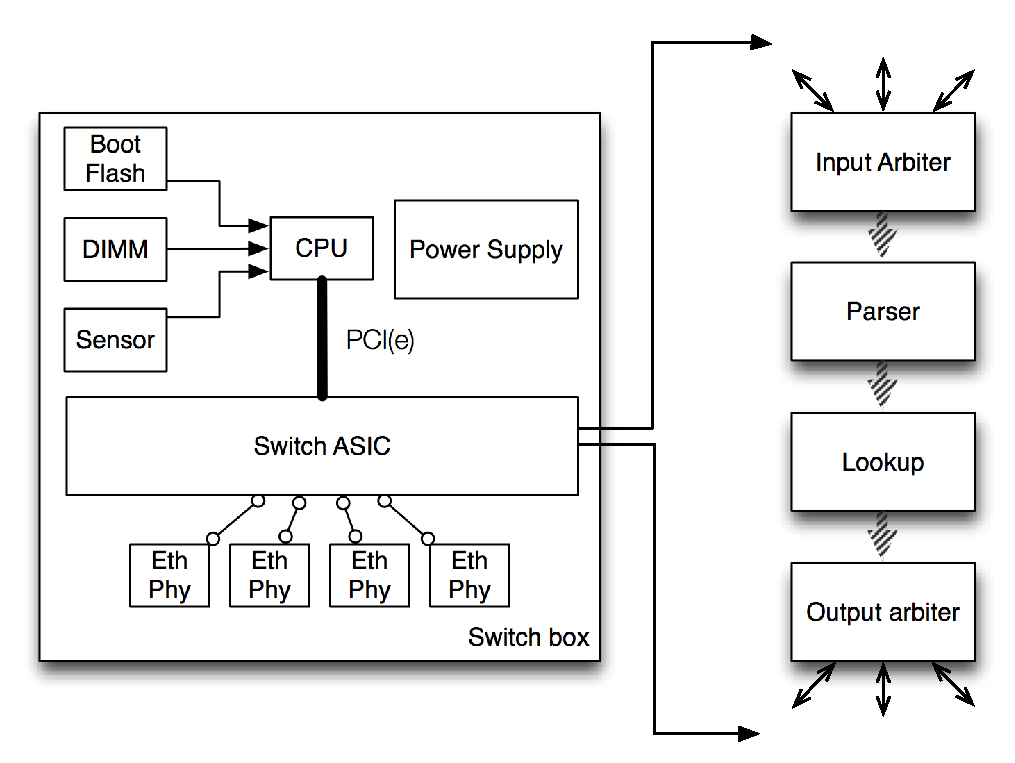
\includegraphics[width=0.6\textwidth]{switch_design}
\caption{A generic architecture of a Switching device.}
\label{fig:background:switch_design}
\end{figure}

Network switches are the main mechanism to multiplex Ethernet links.  This
device type provides collision-free connectivity between network segments.
Switches have multiple functional roles in a network and as a result their
architecture is highly diverse. For example, unmanaged switches provide a low
cost non-configurable interconnection device for small networks, supporting
usually a few 1 gig ports, while distribution switches are used in large
enterprise networks to interconnect aggregation switches, and support multiple
10 or 40 Gig links.  In this section we will use as an architectural example of
a switch, the Top-of-Rack~(TOR) switch.  This switch type is used in datacenter
networks to aggregation traffic between the edge and the distribution network
segments.  TOR switches can forward non-blocking high-rate traffic at line rate,
using a single silicon chip.  As presented in
Figure~\ref{fig:background:switch_design}, a typical switch device consists of
the following components:

\begin{itemize}
  \item \emph{CPU}: Switch boxes contain a programmable CPU, which is used to
        run the control plane logic and provide reconfigurability to users.
        Switch vendors usually use low-power CPUs, such as SoC PowerPC chips or
        even ARM and MIPS CPUs. The CPU can access runtime memory
        module (Boot Flash and RAM), to store transient state, and persistent
        memory (e.g.~SD Cards) through memory extension slots, to store log
        files and configuration. Such CPUs are sufficient to run simple switch
        control-plane functionality, but they are limited to support
        intensive processing tasks. 
  \item \emph{Switch ASIC}: The Application-specific integrated
        circuit~(ASIC)~\cite{hp-asic,broadcom-asic,intel-asic} implements in
        hardware the forwarding plane of the switch.  The capabilities of an
        ASIC are variable, depending on the vendor and the cost, but define the
        performance limits of the device to handle traffic. Implementation
        details of a ASIC silicon remain usually concealed, as they constitute an
        important asset for the producer.  The development of a silicon
        design is a cost and time consuming process which takes years of development and testing
        and requires significant human and material resources. As a result, 
        switch silicon innovation has a high latency to reach the production
        environment. Further, switch silicon face similar limitations as the CPU
        chips. The processing rate is upper bound by the transistor
        density and size. 

        TOR-type switches can handle line-rate non-blocking traffic for a few
        ports, using a single ASIC silicon.  An ASIC contains four important
        modules.  The \emph{input arbiter} module multiplexes and synchronizes
        packets from the Ethernet ports to the main processing pipeline of the
        silicon. The arbiter ensures non-preemptive packet processing, by
        bridging the rate mismatch between the silicon clock and the
        transmission rate of the link.  In the main processing pipeline the ASIC
        requires a \emph{protocol parsing} module and an \emph{address lookup}
        module. The protocol parser extracts significant packet fields from a
        packet and the memory lookup module uses them to define the packet
        processing and forwarding operations.  The lookup module relies on an
        interface with an external memory module in order to match protocol
        fields with forwarding policy.  Memory modules have a trade-off between
        cost and access speed and there is a trade-off between memory cost and
        memory management complexity~\footnote{CAM/TCAM lookup: < 10 clock
          cycles, SRAM: 2-3 nsec, DRAM: 20-35
          nsec,~\url{http://people.ee.duke.edu/~sorin/prior-courses/ece152-spring2009/lectures/6.2.2-memory.pdf}}.
        Finally, the \emph{output arbiter} module is responsible to perform the
        required modifications to the packet and forward it to the appropriate
        output queue. Apart for the mentioned modules, a silicon can have
        additional processing modules to enable extended functionality such as
        access control list (ACL), flow statistics monitoring.

  \item \emph{ASIC-CPU communication}: The switch CPU switching is
        interconnected with the ASIC over a PCI or PCI-express bus. The
        communication channel provides bi-directional communication:
        the firmware controls ASICs registers,
        to define forwarding functionality, and the ASIC propagates exceptions
        to the firmware. The channel provides sufficient bandwidth for
        control plane communication, but the rate is primarily defined by the
        speed of the CPU.
  \item \emph{Memory}: Apart for the in-ASIC memory modules, modern switches
        also use multiple memory types to support the run-time requirements of
        the firmware. A switch usually provides to the CPU Boot Flash,
        to boot the OS/firmware, DIMM RAM and multiple memory slots,
        for switch logging and configuration storage.
  \item \emph{Ethernet ports} : The receipt and transmission of Ethernet packets
        is implemented as a separate hardware circuit. The module is responsible
        to implement the physical layer and MAC layer protocol and propagates
        packets to the ASICs using a  Media Independent Interface (MII).  The
        phy module  usually contains small packet buffers to reduce packet
        losses for bursty traffic.  
\end{itemize}

TOR switches are simple switch devices supporting traffic requirements on the
edges of the network, and support lower to middle forwarding performance. As we
move closer to the core of the network, the requirements for forwarding
performance become higher and device complexity increases. Multi-chassis
switches and routers cannot contain the required functionality in a single
silicon. Packet processing is distributed between multiple silicons and complex
clos interconnection crossbars are used to provide non-blocking terabit
backplane capacity~\cite{juniper_t_series}. In addition, providing fast address lookup
requires multiple distributed buffers and cache coherent protocols to ensure
state consistency~\cite{cisco_cef}. In this classes of devices, the control 
plane abstraction has a complex and slow translation to appropriate management 
of the silicon and flexibility is restricted.  

% Higher-end chassis Switches, employ more complex architectures 
% to support Terrabyte traffic rates, using multi-step packet processing and
% connection redundacy. Because their processing and forwarding capabilities can
% match the capabilities of routers, their architecture is similar to high-end
% switch. 
% An extensive discussion over hardware architecture of
% older high-end Cisco switches is presented in~\cite{cisco-routers}.

\section{Forwarding Control in Production Networks} \label{sec:background:netcontrol}

% In this section, we
% present the Data Link and Network layer protocols used in current production
% networks for dynamic control and discuss their limitations
% 
% \subsection{Routing and switching}

Dynamic network control has been an important functionality for computer network
technologies. Forwarding devices can reconfigure their forwarding logic, when the
network state changes, and thus provide end-to-end connectivity, adjusted to the network
environment. Existing standardized approaches aim for \emph{distributed},
\emph{autonomous} and \emph{resilient} network control and are influenced
extensively by the end-to-end principle of the Internet. A switch or a router
control functionality requires only local forwarding configuration. The device at 
run-time uses a number of well-defined distributed protocols that allow
the reconstruction of the global network configuration, by configuration sharing with
other devices. Using the global network configuration, the
forwarding logic can calculate an optimal forwarding policy and maximize
network performance. Because the state is constructed collectively, the network
provides log-term resilience. If a link is disconnected, the distributed
protocol can propagate this information across the network and devices can
recalculate the optimal policy, while if a device is rebooted, it can rebuild
its global view using only its local configuration. 
In this section we present
existing production-level protocols that enable distributed network control. We
focus on the Data-Link and Network layer protocols as these layer define the
hop-by-hop forwarding.

\subsection{Data-Link Layer Control}

Data-Link layer control protocols provide loop-detection, and VLAN and QoS
automation. Loop detection is used to avoid packet loops in networks with
redundant connectivity, as Ethernet doesn't provide timeout functionality.
Spanning Tree protocol(STP) was a first attempt to addressed this problem,
standardised by IEEE in 802.1D-1998~\cite{ieee_802_1d_1998}. The protocol
implemented the distributed spanning tree construction algorithm presented
in~\cite{Perlman1985}. The algorithm uses broadcast messages to discover a
spanning tree over the graph of the network, with respect to a common root
switch and controls a state machine per port, which disables packet
forwarding when a link is not part of the spanning tree.  Because the initial
definition of the protocol was slow in tree re-calculation after a network
change, IEEE introduce the Rapid Spanning Tree Protocol (RSTP), an evolve
version of STP, in~\cite{ieee_802_1d_2004}.  In addition, a modified version of
the protocol was defined to address the requirements of VLAN functionality. VLAN
tagging can creates multiple subgraphs over the network. The protocol
runs individual STP algorithms each subgraph to construct individual spanning
trees and reduce unnecessary port blocking.
This functionality is provided by IEEE Multiple Spanning Tree
Protocol (MSTP)~\cite{ieee_802_1q}, while Cisco has developed a series of
proprietary protocols~\cite{pvst,pvst+}.  Finally, IEEE has recently defined an
advanced STP protocol that enables switches to discover and use in parallel
redundant network links, in the IEEE 802.1aq standard~\cite{ieee_802_1aq}.

In terms of automatic configuration, network vendors and standardization bodies
have developed a number of protocols that can disseminate information to
neighbouring nodes and ease device management. Such protocols have high churn
between vendors and each vendor defines its custom standard. In this class of
protocols we consider Link Layer Discovery Protocol (LLDP), supported by IEEE,
Cisco Discovery Protocol (CDP),  Extreme Discovery Protocol (EDP) and Nortel
Discovery Protocol (NDP). Finally,in order to reduce the administration burden
of VLAN configuration for inter-switch trunk links, Cisco has developed the 
VLAN Trunking Protocol (VTP).

In the class of Data Link layer protocols we also consider the MPLS
protocol~\cite{RFC3031}. The MPLS technology tries to bridge the gap between
virtual-circuit technologies, like ATM, and packet-switched networks. MPLS
reduces the ATM control plane complexity and removes the limiting small cell
size. MPLS forwarding uses tunnel labels, that simplify the lookup process and
reduces memory requirements. MPLS is used extensively in the distribution layer
of large networks. In order to automate the configuration of MPLS circuits, the
protocol use the LDP protocol~\cite{RFC5036} to setup automatically labels
across the network. In addtion, IETF defined a mechanism to translate RSVP
resource requests to MPLS tunnel configuration~\cite{RFC3209}.  Because MPLS
doesn't provide resource control, the IETF defined the \emph{Autobandwidth}
mechanism.  Autobandwidth monitors tunnel bandwidth requirements and
recalculates paths when bandwidth requirements change. A study on a deployment
of this technology in the MSN network though has highlighted that the allocation
policy is under-optimal for significant periods of the network functionality~\cite{Pathak2011}.

% In Data-Link layer we can also consider the MPLS protocol 

\subsection{Routing control protocols}

In the network layer, modern network technologies exercise control using routing
protocols. Routing protocols follow a similar approach to Data Link layer
protocols and provide mechanisms to disseminate local configuration to the
network. Routing protocols are classified in three categories: \emph{Link
  State}, \emph{Distance Vector} and \emph{Path Vector}. Link state protocols
theory build on-top of the Djikstra algorithm~\cite{Djikstra1959}. Routers
disseminate their local forwarding configuration to the rest of the network.
Using this global state exchange, each router is able to construct the global
connection graph. Each router can use the graph to calculate the minimum
spanning tree of the network, using Djikstra's algorithm.  Currently there is a
plethora of Link State protocol specification in the network community.  IETF
has developed the OSPF protocol~\cite{RFC2328}, an Ipv4 specific routing protocol,
while the Open Systems Interconnection~(OSI) organisation has defined the IS-IS
protocol~\cite{RFC1142}, a network layer agnostic routing protocol.  Link state
routing protocols provide provide high flexibility to define the optimisation
function of the routing system.  Each router has view over the complete graph of
the network and router can propagate multiple link performance indexes
(e.g.~link load, link speed ).  Nonetheless, the optimization function must be
homogeneous across the network, in order to avoid routing loops.

Distance Vector routing protocols employ a different approach to provide
efficient global routing policies. Routing table is constructed using
information from adjacent routers. Network changes are slowly propagated across
the network, through point-to-point information exchanges, until all routers
converge.  Distance Vector protocols use the Belman-Ford
algorithm~\cite{bellman1956} to achieve routing optimality. IETF developed the
RIP  protocol~\cite{RFC2453} to implement Distance Vector routing, while Cisco
has developed the proprietary IGMP protocol~\cite{Rutgers1991}. Distance Vector
protocols are less extensible than Link State routing protocols, but can be
implemented with smaller computational and memory requirements.

Finally, Path Vector routing protocols evolve Distance
Vector protocols to support inter-domain routing. In this class of routing
protocols, adjacent routers advertise the AS path towards for a specific subnet. 
Path Vector routing permits ASes to abstract routing policy details, but provide
sufficient information for the other ASes to define their forward policy. As a
result, the BGP protocol doesn't provide an explicit routing protocol, but
provides a sufficient framework for information exchange.  The BGP
protocol~\cite{RFC1265} is currently the predominant Path Vector routing
implementation.

Due to their distributed nature, routing protocols provide long-term routing
resilience, while their mathematical foundation is to provably correct.
Nonetheless, the control abstraction of these protocol is not a good fit for
administrator to exercise dynamic control in the network. For example, it is
intractable for a network manager to speculate on the impact of network policy
changes.  In 2008 the global Internet was severely affected by a BGP
misconfiguration from the Pakistani national ISP in an effort to control traffic
from YouTube service~\cite{bgp_config_error}.  In addition,
routing inconsistencies during routing changes can impact significantly network
performance.  For OSPF, authors in~\cite{Watson2003} monitor OSPF functionality
in a regional ISP and report high churn in routing even during periods without
significant network events, while the latency to converge after a network change
is on average on the order of seconds. Similar results have been observer in
BGP\@. In~\cite{Kushman2007} the authors highlight a strong correlation of BGP
instability and VoIP performance. 

\section{Programmable Network Control}

Because of the limitation of current standardized network control frameworks,
the research community over the years has proposed a number of interesting
approaches for network control evolution. In this section we present the three
most significant and complete approach to this problem, namely Active Networks,
Devolved Control of ATM Networks and Software Defined Networking. 

\subsection{Active Networks}

The problem of protocol ossification in the network layer and the requirement
for network evolution, was highlighted  by the network research community since
mid 90's. In~\cite{O'Malley1992}, the authors argue on the generality of the
7-layer OSI network abstraction. They claimed that the networks functionality
should be more dynamic and forwarding devices should be able to accommodate
variable number of protocol layers. In their work they present an extensible
protocol modeling framework to layer protocol processing. Motivated by these
observations, DARPA funded the \emph{Active Networks}
project~\cite{darpa_active_net}, in an effort to develop next generation network
devices that can accommodate seamlessly new protocol functionality. 

Active networks modify the default packet processing mechanism and introduce the
notion of \emph{capsules}. Capsules are network packets that carry data, as
well as, processing code. On each hop, the default packet processing logic is
extended with the code contained in the capsule, thus redefining network
functionality. This network processing approach provided user-driven protocols
upgrades, without a requirement for devices upgrade.  In addition, the
development of novel programming languages, like Java, provided the
building blocks to implement code distribution frameworks.

Research in active networks tried to define two mechanisms : the \emph{capsule
  API and format} and the \emph{switch architecture}. In terms of capsule
format, the active network community defined the Active Network Encapsulation
Protocol~(ANEP)~\cite{alexander1997a}.  ANEP, through its format specification,
made a clear separation between functionality and data. An Active Node using a
new protocol would inject firstly new processing logic, using code capsules, and
then send the data stream, as data capsules.  The format was adopted by the ANTS
and Sprocket frameworks.  Sprocket~\cite{Schwartz2000} was an effort to develop
an efficient capsule programming language by BBN technologies. The language uses
a restricted set of the C language, avoiding any security vulnerable structures
like pointers, while it introduced native support for SNMP browsing. Sprocket
compiled source code to compact MIPS assembly. Each switch would receive code
capsules and run the code in a MIPS virtual machine. The VM could not persist
any state on the switch, but it was able to modify the data section of a packet.
Sprocket provided secured injected code with a public key secure hash of the
code binary, but without sufficient details on the authentication logic.
ANTS~\cite{Wetherall1998} was an attempt by the Active Networks group in MIT to
develop a sufficient capsule programming environment.  ANTS uses a restricted
version of the Java language to program capsules, because of the inherent object
serialization functionality of Java, while the processing logic is defined
through a small set of Java interfaces. ANTS permits injected code to persist
flow state on a switch and modify packet content. An interesting extension of
the ANTS framework was the code dissemination mechanism. An end-node deployed
new protocol functionality solely to the local Internet gateway, and the code is
forwarded along with the packets to each next-hop. Finally, The university of
Pensylvania active networks group developed its own approach to capsule
programming.  PLAN~\cite{Hicks1998} used a restricted version of the OCaml
language to abstract capsule access to the local switch state and implement
custom forwarding logic. PLAN did not follow the ANEP packet format. A PLAN
capsule contains code and data and the code section replaces the network header
information. In order to secure switch infrastructure, the language disallowed
packet data modification or switch state persistence.  Ultimately, the language
provided a framework for programmable control plane.

In terms of Active Network platform architecture, the community developed a
number of architectures, addressing multiple aspects of efficiency in capsule
processing. University of Pensylvania proposed the SwitchWare Execution
Environment (EE)~\cite{Alexander1998}.  The architecture defined an OCaml module
framework for capsule processing. A core focus of the SwitchWare EE was strong
multi-dimension security for active networks, both on the local system, as well
as, during capsule execution.  SwitchWare used SANE~\cite{Alexander1998b}, a
trustworthy operating system, to secure the functionality of the switch, and
build on top of its security primitive higher level of trust. The platform
addressed issues regarding secure execution and authentication, as well as,
capsule code verification.  PLANet~\cite{Hicks1999} and Active
Bridge~\cite{Alexander1997b} used the SwitchWare framework to implement novel
functionality in active networks. 

The active networks group in University of Arizona proposed its custom approach
to high performance active network forwarding. Their approach relies on the Scout
OS~\cite{Montz1995}, a communication-oriented OS supporting efficient
layered data processing. On top of Scout, the group developed the Liquid Software
API~\cite{Hartman1999}. The integration of Liquid Software API and Scout, aimed to
establish a tight integration between the OS and the JVM and improve capsule
processing, using the JIT JAVA compiler. 

The CANEs project~\cite{Chae2002} from Georgia Tech Active Networks groups
followed a different approach for the problem and designed a system which
enabled multi-protocol packet processing. CANEs defined a number of
abstractions, which enabled active network applications to stack multiple
protocol processors on the forwarding path. CANEs project build on top of the
Bowman Switch OS~\cite{merugu1999} and established a simple and efficient
abstraction over the Switch resources. 

Researchers from the Columbia University, presented the NetScript switch
abstraction~\cite{daSilva2001}. NetScript is a new programming language
optimized for flexible protocol processing definition and composition. The
project defines three types of protocol composition: layered composition,
composition through protocol bridging and end-to-end composition. Netscript
provides developers the ability to builf flexible extension in existing protocol processing. 

Finally, a joint effort between the Network Laboratory of ETH and the University
of St. Louis, developed a hybrid hardware and software approach for high
performance capsule processing. The High Performance Active Network Node (ANN)
switch architecture~\cite{Decasper1999} proposes the introduction of an FPGA for
each ATM interface which handles capsule execution. Using this infrastructure,
the researchers where able to run the ANTS EE and develop an IPv4 and IPv6
protocol processor to run in Gigabit rates. 

Active network research put forward a number of interesting insights on the
controllability and evolvability problem in computer network functionality.
Nonetheless, their complex and clean-slate approach, reduced their applicability
in production environments. In addition, Active Network functionality was highly
benefited from the relatively low rate of the network rates of the time. CPU
processing capability of the time was able to accommodate the respective link
rates. The rapid evolution of data rate in Ethernet interfaces to Gigabit
speeds, through, makes impossible the development of programmable forwarding
platforms with line rate performance. 

\subsection{Devolved Control of ATM Networks}

\begin{figure}
  \begin{center}
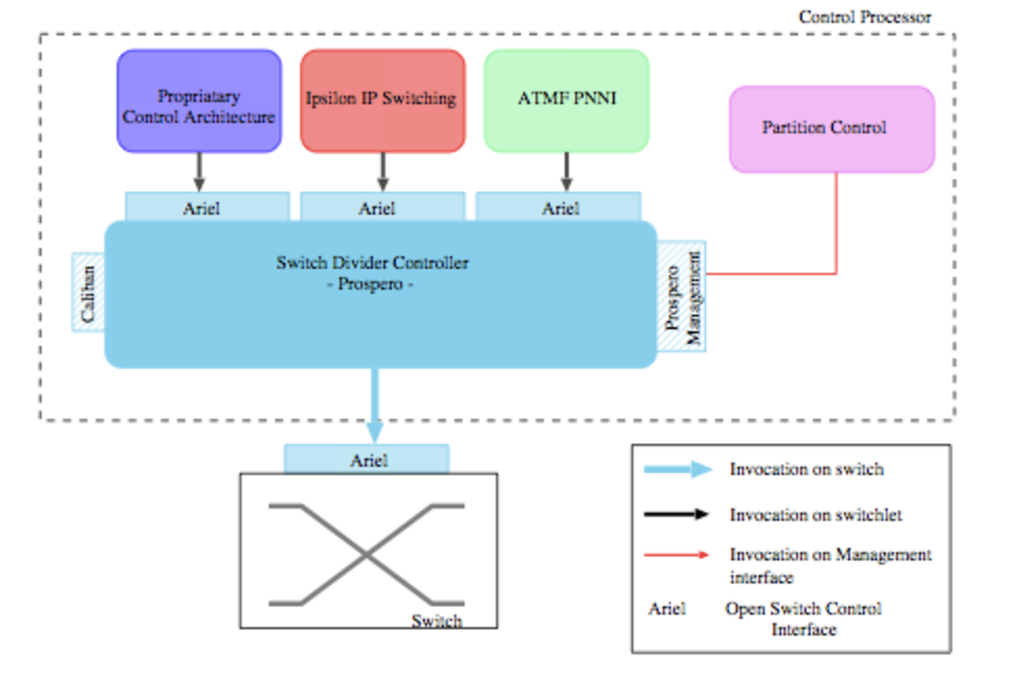
\includegraphics[width=0.7\textwidth]{tempest_arch}
\caption{Tempest switch architecture~\cite{UCAM-CL-TR-450}}
\label{fig:background:tempest_arch}
\end{center}
\end{figure}

\todo{add GSMP protocol reference}
An effort for network programmability in ATM network was also developed in the
University of Cambridge, as part of the DCAN~(Devolved Control ATM Networks)
project~\cite{dcan}.  The system, called Tempest~\cite{Rooney1998}, aimed to
provide dynamic network control and resource virtualization. Tempest provides a
clear separation between the control and forwarding plane of a network device.
The control plane of network devices, is centralised in a single programmable
entity, which implements intelligent and dynamic forwarding.  The implementation
of Tempest is logically divided between three abstractions, depicted in
Figure~\ref{fig:background:tempest_arch}. The Figure presents how a single
switch is able to function in parallel as an IP router, an ATM switch and a
Hollowman controlller~\cite{Rooney1997}, a devolved ATM control framework. 

\paragraph{Prospero Switch Divider} 

The \emph{Prospero} abstraction provides a mechanism to virtualise ATM switch
resources. Prospero provides a resource control interface, which can divide
switch resource between multiple virtual switches, called \emph{switchlets}.  A
switchlet controls a subset of the switch ports, VCI and VPI mappings, packet
buffer and bandwidth. For packet buffer and bandwidth virtualization, Prospero
uses the ATM defined QoS  principles. In addition, Prospero is responsible to
map the control interface, exposed to controllers, with the underlying switch
functionality. 

\paragraph{Ariel Switch Independent Control Interface} 

Switchlets expose forwarding control through the Ariel Interface. Ariel
Interface organises network control through five control objects:
\emph{Configuration}, \emph{Port}, \emph{Context}, {\it Connections}
\emph{Statistics} and \emph{Alarms}.  Configuration provides details for the
switch configuration, Port provides primitive controllability of ports
(e.g.~state, loopback functionality), Context enables QoS policy control,
Connections expose control of VPI/VCI mappings, Statistics exposes packet and
byte counters and Alarms push state change notifications to the controller. Any
Tempest switch runs an Ariel server and translates Ariel request to Prospero
control requests. 

\paragraph{Caliban Switch Management Interface}

Apart from control capability support, Tempest also supported evolved network
management, through the Caliban interface. The interface functionality is
similar to the SNMP protocol. Caliban provides fine level SNMP-style
information, but can also provide higher level aggregation operations over the
switch state. 

In addition to the redefinition of the network control abstraction, Tempest also
proposed a relaxed network resource management scheme.  Specifically, the
architecture proposed a measurement-based admission control mechanism for
circuit establishment~\cite{Lewis1998}. The measurement scheme redefined the
static resource allocation scheme in ATM network, and used effective bandwidth
measurement techniques to estimate available resources.  This admission control
scheme provided higher utilisation of network resources, while providing QoS
guaranteed. 

Tempest defined a highly efficient network control abstraction. The
effectiveness of the control abstraction motivates modern network control
approaches, like SDN, to reimplement it over Ethernet devices.  In addition, the
simplicity of the control abstraction, permitted integration of the technology
with existing forwarding devices  and enabled line rate forwarding and efficient
resource control.  Nonetheless, its strong reliance on the ATM technology made
the approach less relevant for the modern Ethernet-dominated networks~\cite{Crosby2002}. 

\subsection{SDN}\label{sec:background:sdn} 

A recent attempt to develop a framework for distributed and scalable control is
the Software Defined Networking (SDN) paradigm. SDN~\cite{sdn} propose the clean
separation between the control and the forwarding plane of a network device. The
control plane logic is implemented in a separate programmable device and a well
defined protocol establishes the inter-connection between the two devices. 

The SDN approach was highly motivated by relevant earlier attempts in network
programmability(Active Networks and DCAN), but follows an evolutionary approach.
SDN supports existing network data protocols but enables the development of
custom forwarding mechanisms.  The paradigm is motivated by two observations in
current network technologies.  Firstly, the evolution of computer networks has
reduced the applicability of the multi-layer network abstraction. Production
networks contain middleboxes (e.g.~firewall, NAT, layer-5 switches) that operate
on multiple layers of the network and engage extensively in layer violation.
Such devices cannot integrate with existing control mechanisms, while they
remain transparent by the end-hosts. The SDN paradigm aims to provide a new
unifying cross-layer control model that can accommodate such control approaches.
Secondly, although network complexity has increased, network devices still use
stand-alone configuration mechanisms (e.g.  remote logic, CLI interfaces) and
network policies must be decomposed by network administrators in individual
network device policies to fit the existing control abstraction. In order to
modify network-wide configuration, network administrators must login over telnet
or use a web interface to configure each device manually.  In addition, network
vendors develop proprietary control protocols which reduce device interoperable.
SDN enables management centralisation, while the flexibility of the control
abstraction can create new innovating control mechanisms that match network
environment requirements.

The SDN paradigm was highly successful in the network community and within a few
years since its introduction, network vendors engaged in the development of
production-level implementations. In addition, the research community has
developed a number of interesting SDN architectures which address several network
problems. The \of protocol is currently the pre-dominant implementation of the SDN 
paradigm.

\subsubsection{\of protocol} 

\begin{figure}
  \begin{center}
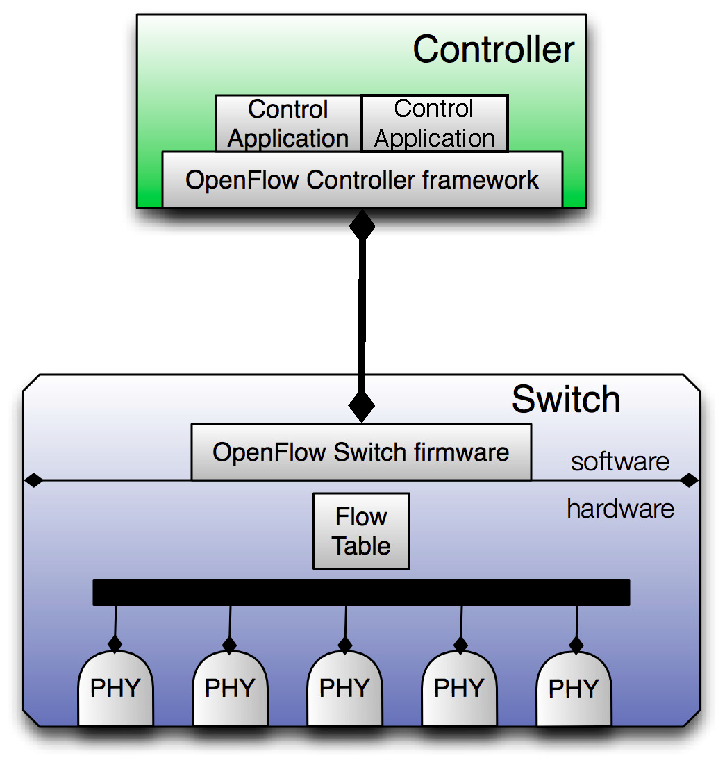
\includegraphics[width=0.5\textwidth]{openflow-schema}
\caption{A schematic representation of a basic \of setup}
\label{fig:background:openflow-schema}
\end{center}
\end{figure}
\begin{table}
  \begin{minipage} []{0.49\textwidth} 
    \begin{tabular}{|p{4cm}  | p{2cm} |} 
      \hline
      Field & OpenFlow Version \\ 
      \hline
      src \& dst MAC addr. & 1.0~\footnote{SInce version 1.1 the protocol
        permits masked mac address matching} \\ \hline
      input port & 1.0 \\ \hline
      VLAN ID & 1.0 \\ \hline 
      VLAN PCP & 1.0 \\ \hline
      MPLS label & 1.1 \\ \hline
      MPLS class & 1.1 \\ \hline 
      IPv4 src/dst addr. & 1.0 \\ \hline
      IPv4 proto & 1.0 \\ \hline
      ARP opcode & 1.0 \\ \hline 
      ARP src/dst IPv4 address & 1.0 \\ \hline 
      ARP src/dst MAC address & 1.2 \\ \hline 
    \end{tabular}
  \end{minipage}
  \begin{minipage} []{0.49\textwidth} 
    \begin{tabular}{|p{4cm}  | p{2cm} |} 
      \hline
      Field & OpenFlow Version \\  \hline
      IPv4 ToS & 1.0 \\ \hline 
      ICMPv4 Type \& Code & 1.0 \\ \hline
      TCP/UDP/SCTP src/dst port & 1.0 \\ \hline
      metadata & 1.1 \\ \hline
      IPv6 src/dst addr. & 1.2 \\ \hline
      IPv6 flow label & 1.2 \\ \hline
      ICMPv6 type \& code & 1.2 \\ \hline
      ICMPv6 Network Discovery target address & 1.2 \\ \hline
      ICMPv6 Network Discovery src/dst MAC address & 1.2 \\ \hline
    \end{tabular}
  \end{minipage}
    \caption{\of tuple fields} \label{tbl:background:openflow_tupple}
\end{table}
  \begin{table}
  \begin{minipage} [b]{0.49\textwidth} 
    \begin{tabular}{| p{4cm} | p{6cm}  | p{1.5cm} |} 
      \hline
      Field & operation & OpenFlow Version \\ \hline
      OUTPUT & output packet to a port & 1.0 \\ \hline
      SET\_QUEUE & output packet to a port queue & 1.0 \\ \hline
      SET\_VLAN\_VID & modify VLAN id & 1.0 \\ \hline 
      SET\_VLAN\_PCP & modify VLAN PCP & 1.0 \\ \hline
      SET\_DL\_SRC SET\_DL\_DST & modify src/dst mac addr. & 1.0 \\ \hline
      SET\_NW\_(SRC,DST) & modify IPv4 src/dst addr. & 1.0 \\ \hline
      SET\_NW\_TOS & modify IPv4 ToS & 1.0 \\ \hline
      SET\_NW\_ECN & modify IPv4 ECN bits & 1.1 \\ \hline
      SET\_TP\_(SRC,DST) & modify TCP/UDP/SCTP src/dst port & 1.0 \\ \hline
      COPY\_TTL\_(OUT,IN) & copy TTL value for IPv4 tunnels & 1.1  \\ \hline
      SET\_MPLS\_LABEL & modify MPLS label & 1.1 \\ \hline
      SET\_MPLS\_TC & modify MPLS traffic class & 1.1 \\ \hline
      (SET,DEC)\_MPLS\_TTL & modify/decrement MPLS TTL & 1.1 \\ \hline
      (PUSH,POP)\_VLAN & Add/remove a VLAN header & 1.1~\footnote{\of 1.0 defined
        a primitive to remove a VLAN header only} \\ \hline
      (PUSH,POP)\_MPLS & add/remove MPLS tag & 1.1 \\ \hline
      (SET,DEC)\_NW\_TTL & modify/decrement IPv4 TTL value & 1.1 \\ \hline
      (PUSH,POP)\_PBB & remove/add a PBB service tag & 1.3 \\ \hline

    \end{tabular}
  \end{minipage}
  \caption{\of available packet actions} \label{tbl:background:openflow_actions}
\end{table}




\of is an instantiation of the SDN paradigm. The protocol was originally
developed by the \of Consortium, a collaborative organisation of academic
institutes, but soon its development was adopted by the ONF, a standards
definition committee comprised of academic institutions and network vendors. \of has
been a highly successful approach to network control. A number of vendors
has introduced support of the protocol in their products
while there are already \of deployments in enterprise networks~\cite{google_of,Kobayashi:vn}.

A representation of a simple \of topology is presented in
Figure~\ref{fig:background:openflow-schema}. A minimum \of topology consists of
two entities: the \emph{Controller} and the \emph{Switch}. The Controller
implements and disseminates the control logic of the network to the switches
over a control channel. A controller can control multiple switches. In addition, 
the network community has developed a number of programming environments to
develop \of control applications. Such programming environments provide a 
higher level abstraction over the \of protocol and reduce the exposure of
the developer to the run-time details~\cite{nox,floodlight,nodeflow}.

The switch entity is responsible to transform \of protocol operations in data
path policy modifications. The \of functionality is split between the data and
control layer of the switch. In the data layer, the protocol implements a simple
packet processing algorithm.  For each packet, the hardware extracts a number of
fields and matches them against the entries of a \emph{Flow Table}.  The Flow
Table is a memory abstraction which contains forwarding policy. It comprises of
flow entries which conceptually consist of three parts: the flow tuple, the flow
statistics and the flow action list.  The flow tuple synthesizes a flow
description using all the significant packet header fields.  We present the list
of fields in Table~\ref{tbl:background:openflow_tupple}.  The protocol
associates with each flow tuple a flow mask, which permits field wildcarding in
a flow definition.  Flow statistics store flow packet and byte counters. The
action list, contains the list of actions that should be applied on every
matched packet.  We present in Table~\ref{tbl:background:openflow_actions} the
packet processing actions defined by the \of protocol.  On a packet reception,
if a matching flow is found in the flow table, then the flow statistics are
updated and the action list is applied on the packet. If there aren't any
matching flow entries, the packet propagates as an exception to the control
layer of the switch.  The control plane of the switch implements the translation
of the \of protocol into data path modifications.  It provides access and
modification functionality to the switch configuration and the flow table. The
switch is able also to propagate autonomously information and exceptions 
to the controller. 

The ensemble of a flow table and a set of switch ports comprises an \of
\emph{datapath} and is the core abstraction for network control.  The protocol
defines a number of protocol message types to manage datapath resources. \of 
control operations can be grouped in two categories:
\emph{Forwarding control} and \emph{Switch configuration}. In the rest of the
section we present how this functionality is addressed by \of messages and how
this mechanism is evolved over the different versions of the protocol. We
focus our protocol presentation over the 1.0 version of the protocol.
ONF has releases three revisions of the
protocol, version 1.1, 1.2 and 1.3, which change significantly the protocol
specification. Nonetheless, the majority of production systems are predominantly 
version 1.0 compliant.
% the \of protocol version 1.0 to control a
% network. This version was introduced in 2009 and is currently the market default
% support. Since then, the ONF steering board has released three more version,
% 1.1, 1.2 and 1.3, which redefine to a great extend the default processing logic
% of the abstraction. Following, we will present the core mechanisms of version
% 1.0 and describe in a higher level the incremental differentiations introduced
% in the following versions of the protocol. 

\paragraph{Forwarding control}

\of provides fundamentally two modes of control: \emph{reactive} and 
\emph{proactive} control. In the reactive approach, the switch is configured to
forward every unmatched packet to the controller, and the controller is
responsible to respond with appropriate modification in the flow table. The
protocol defines the {\tt pkt\_in} message type, that can propagate the header
of a packet to the controller, and the {\tt flow\_mod} message type, that can
manipulate flow table entries. The reactive control approach provides 
fine control over the traffic dynamics, but, depending on the deployment
environment, can introduce significant load on the control plane. In the proactive
approach, the controller is responsible to pre-install all required flows in the
flow table and avoid any packet handling exceptions. Because this approach
lucks data plane feedback, the \of protocol provides the {\tt stats\_req/stats\_resp}
and {\tt aggr\_stats\_req/aggr\_stats\_resp} message types. These message types allow
the controller to poll dynamically for flow statistics and infer network
resource allocation. In order to ensure atomicity in the protocol, the protocol
also define a {\tt barrier\_req/barrier\_reply} message type, which provides a synch 
point between the controller and the switch. A {\tt barrier\_reply} is send by a
switch as a response to a {\tt barrier\_req} from the controller, only if all previous 
operations are processed. 
Finally, the \of protocol provides two additional message
types to increase users ability to interact with the forwarding plane: the {\tt
  pkt\_out} and the {\tt flow\_removed}. The {\tt pkt\_out} message enables the
controller to inject traffic in the data plane and the {\tt flow\_removed} message
can notify the controller when a flow entry is removed from the flow table. The
protocol defines flow timers and the switch can remove a flow with an expired
timer. 

\paragraph{Switch configuration} 

Apart from the control of the flow table, the \of protocol provides switch
configuration capabilities. A controller can use the {\tt
  switch\_config\_req/switch\_config\_resp} message types, to discover switch \of
operation support.  In addition, the protocol provides capabilities to control
port state with the {\tt port\_mod} message type. The switch is also able to
notify the controller when a port changes its state (e.g.~link is detected to be
inactive in the physical layer) with the {\tt port\_status} message. In the
recent revisions of the protocol, the steering committee has introduced the
capability to control per port traffic shaping queues. 

\paragraph{Protocol evolution} 

Since the specification of the version 1.0 of the protocol, the steering
committee of the protocol has produced 3 non-backward compatible revisions of
the protocol. The updates in the protocol are motivated both by the osmosis
between the hardware and software \of community, as well as, by the introduction
of new deployment use cases. 

Version 1.1 of the protocol introduces a number of new features for
integration of the protocol with the silicon functionality. Firstly, the
default packet processing algorithm is modified. A switch can accomdate multiple
flow tables and the lookup process searches sequentially each of the
tables for flow matches. The packet must have a match in each of the tables
otherwise a {\tt pkt\_in} message
is generated. In addition, in order to persist partial results between
tables, the protocol define a 64-bit metadata field and the
action list is augmented with operations over the metadata field, as well
as, over the table search process (e.g.~terminate lookup, skip table).
Secondly, the protocol introduces a primitive to express multipath support in
the protocol. This functionality is exposed through a group table abstraction.
Group table entries contain a set of buckets containing flow actions and an
assigned output port. A controller in the action of a flow can 
forward packet to a group entry. The goup selection action can select to forward
the packet either to all the buckets of the entry (ALL) or select randomly a
bucket, in a manner similar to the Equal Cost Multiple Path routing
(ECMP)~\cite{RFC2992} functionality, (SELECT) or select a specific bucket
(INDIRECT) or forward packet to the first group entry for which the output port
can forward packet (FAST\_FAILOVER).  Thirdly, the protocol introduces MPLS
matching support and manipulation.

Version 1.2 of the protocol augments further protocol functionality. This
revision introduces support for IPv6 and Provider Bridge Network (PBB -
Mac-in-Mac) traffic. In addition the protocol defines a new TLV format for flow
Match definition, in order to relax the \of tuple definition.  Finally, the
protocol defines a model to control multiple controller access to the switch.
Multi-Controller schemes provides resilience to the control of the network. 

In Version 1.3 the protocol definition introduces protocol support of QoS
control. The protocol defines a new table abstraction, the metering table, which
contains queue definitions. In addition, this protocol definition introduces the
idea of multiple parallel control channels towards the same controller, in order
to paralelise {\tt pkt\_in} transmission, and defines a mechanism to suport
message fragmentation.  

Because the recent versions of the protocol has become complex, the vision of
future \of deployment, is to differentiate switch abstraction and develop
diverse product ranges that will provide optimized support for a subset of the
protocol. 

\section{Control Plane Applications} \label{sec:background:ofapp}
% \subsection{Datacenter network}
% \subsection{Home network}
% \subsection{Wireless network}
% \subsection{Simulation}

\section{Conclusions}
